\chapter{Resultados}
\label{ch:resultados}

Para a aplicação dos controladores \acrshort{mpc} criados nos capítulos anteriores, foi desenvolvido um
ambiente \textit{Simulink} (\cref{fig:simulinkusingmpc}) onde cada um dos diferentes controladores obtidos
foram conectados ao \acrshort{tclabsp} para realizar seu controle.

Todos\footnote{
    O \acrshort{matlab} não conseguiu criar um controlador baseado no modelo experimental Box-Jenkins
    pois este modelo possui pólos discretizados próximos de $z=0$.
}  os diferentes controladores foram submetidos aos mesmos sinais de referência (\textit{set-point})
e ao mesmo tempo de experimento. Os sinais de referência utilizados foram sinais de amplitude randômica
e com duração de duas vezes o tempo de acomodação da planta em malha aberta, ou seja, $2$ x $T_s = 2$ x $383s = 766s$.
A duração do experimento foi determinada de forma que cinco sinais de entrada distintos pudessem ser
aplicados ao sistema, sendo assim o tempo dos experimentos foi de $5$ x $766s = 3830s$.
Cada um dos experimentos foi repetido ao menos 3 vezes e ao final foi calculada uma média de todos os 
sinais coletados para atenuar possíveis erros pontuais de cada experimento.

\begin{figure}[!h]
	\caption{Ambiente Simulink para implementação dos controladores MPC}
	\begin{center}
		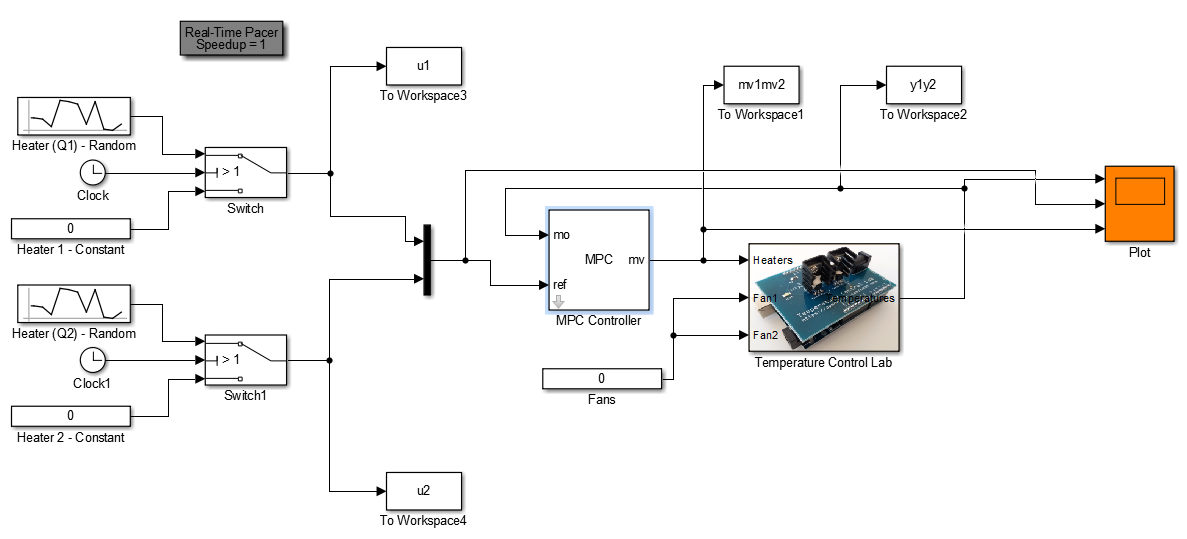
\includegraphics[width=1.00\textwidth]{./5_images/SimulinkUsingMPC.png} 
		\label{fig:simulinkusingmpc}
	\end{center}
	\centering
	\makebox[\width]{Fonte: Autor} 
\end{figure}

As \crefrange{fig:resultadosmpc-teoss}{fig:resultadosmpc-exparx} apresentam os gráficos de resposta em malha fechada
para cada um dos experimentos aplicando os modelos obtidos.

Para fins comparativos, a \cref{fig:resultadospid} apresenta o gráfico de resposta do controlador
\acrshort{pid} apresentado na \cref{sec:controlador_pid} e a \cref{tab:resultados_mpc_e_pid}
apresenta os valores de \textit{fit} (\cref{eq:nrmse}) dos controladores \acrshort{mpc} e \acrshort{pid} 
comparando-os com os sinais de referência (\textit{set-points}).

\begin{figure}[!h]
	\caption{Resposta do controlador MPC criado a partir do modelo teórico}
	\begin{center}
		\includegraphics[width=1.00\textwidth]{./5_images/ResultadosMPC-TeoSS.eps} 
		\label{fig:resultadosmpc-teoss}
	\end{center}
	\centering
	\makebox[\width]{Fonte: Autor} 
\end{figure}

\begin{figure}[!h]
	\caption{Resposta do controlador MPC criado a partir do modelo experimental (função de transferência)}
	\begin{center}
		\includegraphics[width=1.00\textwidth]{./5_images/ResultadosMPC-ExpTF.eps} 
		\label{fig:resultadosmpc-exptf}
	\end{center}
	\centering
	\makebox[\width]{Fonte: Autor} 
\end{figure}

\begin{figure}[!h]
	\caption{Resposta do controlador MPC criado a partir do modelo experimental (ARMAX)}
	\begin{center}
		\includegraphics[width=1.00\textwidth]{./5_images/ResultadosMPC-ExpARMAX.eps} 
		\label{fig:resultadosmpc-exparmax}
	\end{center}
	\centering
	\makebox[\width]{Fonte: Autor} 
\end{figure}

\begin{figure}[!h]
	\caption{Resposta do controlador MPC criado a partir do modelo experimental (Output-Error)}
	\begin{center}
		\includegraphics[width=1.00\textwidth]{./5_images/ResultadosMPC-ExpOE.eps} 
		\label{fig:resultadosmpc-expoe}
	\end{center}
	\centering
	\makebox[\width]{Fonte: Autor} 
\end{figure}

\begin{figure}[!h]
	\caption{Resposta do controlador MPC criado a partir do modelo experimental (espeço de estados)}
	\begin{center}
		\includegraphics[width=1.00\textwidth]{./5_images/ResultadosMPC-ExpSS.eps} 
		\label{fig:resultadosmpc-expss}
	\end{center}
	\centering
	\makebox[\width]{Fonte: Autor} 
\end{figure}

\begin{figure}[!h]
	\caption{Resposta do controlador MPC criado a partir do modelo experimental (ARX)}
	\begin{center}
		\includegraphics[width=1.00\textwidth]{./5_images/ResultadosMPC-ExpARX.eps} 
		\label{fig:resultadosmpc-exparx}
	\end{center}
	\centering
	\makebox[\width]{Fonte: Autor} 
\end{figure}

\begin{figure}[!h]
	\caption{Resposta do controlador PID auto-sintonizado}
	\begin{center}
		\includegraphics[width=1.00\textwidth]{./5_images/ResultadosPID.eps} 
		\label{fig:resultadospid}
	\end{center}
	\centering
	\makebox[\width]{Fonte: Autor} 
\end{figure}

\begin{table}[!h]
	\centering
	\caption{Qualidade dos controladores \acrshort{mpc} e \acrshort{pid}}
	\label{tab:resultados_mpc_e_pid}
	\begin{tabular}{l|cc|c} \toprule
		{Modelo utilizado no controlador}              			            &	{\textit{Fit} Sensor 1}	    &	{\textit{Fit} Sensor 2}     & {\textit{Fit} médio}			    \\ \midrule
		MPC Teórico \acrshort{ss} (\cref{eq:tclab_modelo_teorico})	        &   $45.84\%$                   &   $44.07\%$                   &   $44.95\%$                       \\ 
		MPC Experimental \acrshort{oe} (\cref{tab:tclabsp-model-oe})	    &   $44.35\%$                   &   $40.57\%$                   &   $42.46\%$                       \\ 
		MPC Experimental \acrshort{armax} (\cref{tab:tclabsp-model-armax})	&   $39.92\%$                   &   $42.50\%$                   &   $41.21\%$                       \\ 
		MPC Experimental \acrshort{tf} (\cref{tab:tclabsp-model-tf})		&   $40.25\%$                   &   $34.55\%$                   &   $37.40\%$                       \\ 
		MPC Experimental \acrshort{ss} (\cref{eq:tclabsp-model-ss})			&   $38.55\%$                   &   $33.57\%$                   &   $36.06\%$                       \\ 
		MPC Experimental \acrshort{arx}	(\cref{tab:tclabsp-model-arx})		&   $43.71\%$                   &   $27.33\%$                   &   $35.52\%$                       \\ 
		PID (\cref{tab:pid_values})	                                        &   $40.13\%$                   &   $26.44\%$                   &   $33.28\%$                       \\ \bottomrule 
	\end{tabular}
	\caption*{Fonte: Autor}
\end{table}
